\documentclass[conference]{IEEEtran}

% ==============================================================
%  PACKAGES
% ==============================================================
\usepackage{cite}
\usepackage{amsmath,amssymb,amsfonts}
\usepackage{graphicx}
\usepackage{textcomp}
\usepackage{xcolor}
\usepackage{booktabs}
\usepackage{array}
\usepackage{url}

\def\BibTeX{{\rm B\kern-.05em{\sc i\kern-.025em b}\kern-.08em
    T\kern-.1667em\lower.7ex\hbox{E}\kern-.125emX}}

% Set Keywords title instead of Index Terms
\renewcommand\IEEEkeywordsname{Keywords}

\begin{document}

% ==============================================================
%  TITLE & AUTHORS
% ==============================================================
\title{Phase2Net: A Dynamic Feature Selection and Two-Phase Online Adversarial Training Framework for Robust Network Intrusion Detection}
\author{}
\maketitle

% ==============================================================
%  ABSTRACT & KEYWORDS
% ==============================================================
\begin{abstract}
Machine learning based Network Intrusion Detection Systems (NIDS) in cloud environments remain vulnerable to adversarial evasion attacks that manipulate network flow features. Existing defenses may reduce clean traffic performance or rely on static adversarial retraining, where pre-generated perturbations can become less effective as model parameters change. This paper proposes Phase2Net, a joint defense framework combining Adversarial Stability SHAP feature selection with dynamic online Projected Gradient Descent (PGD) training. The proposed method selects 27 features based on an Adversarial Stability Score and generates fresh adversarial perturbations for each mini-batch during training. Evaluated on 1,264,001 test flows from the CSE-CIC-IDS2018 dataset across three random seeds, Phase2Net achieves 96.19\% clean accuracy and 90.13\% accuracy under PGD-100 attacks, demonstrating improvements of 3.37 and 16.23 percentage points over the undefended baseline, respectively. The model also maintains robustness against unseen white-box, black-box, and transfer attacks, with an average time below 0.02\,ms per flow.
\end{abstract}

\begin{IEEEkeywords}
Network Intrusion Detection, Adversarial Machine Learning, Adversarial Training, SHAP, Feature Selection, Cloud Security.
\end{IEEEkeywords}

% ==============================================================
%  SECTION I — INTRODUCTION
% ==============================================================
\section{Introduction}

\subsection{Problem Context}
Network security is important for protecting modern digital systems and services. To protect these systems from threats such as Distributed Denial of Service (DDoS), brute force attacks, and web exploits, cloud providers use Network Intrusion Detection Systems (NIDS). Machine learning (ML) and deep learning (DL) models are widely used in NIDS. They analyze network flow features extracted by tools such as CICFlowMeter from benchmarks such as CSE CIC IDS2018~\cite{ref1,ref2}. Deep neural networks can achieve high detection accuracy on clean traffic. However, they are at risk to adversarial evasion attacks~\cite{ref3}. Attackers make tiny changes to network data to hide from security without causing suspicion. So, clean accuracy alone is not enough to benchmark NIDS security.

\subsection{Problem and Motivation}
Implementation of robust deep learning classifiers in cloud networks creates three challenges:
\begin{itemize}
    \item Clean Accuracy vs.\ Robustness Trade off: Training a model to be more secure against adversarial can lower its accuracy on normal traffic. This can lead to more false alarms.
    \item Static Attack Dependence: Common defense methods use static data augmentation~\cite{ref4}. They add pregenerated attack examples in the training data. But as parameters of the model changes, these samples become less effective. This can make the model vulnerable to new attack patterns~\cite{ref5}.
    \item Incomplete Robustness Evaluation: Many NIDS defenses are tested primarily against single step attacks or the attack used in training. This makes their performance against unseen iterative, black box, and decision-based attacks less obvious.
\end{itemize}

\subsection{Research Gap}
Previous research has investigated adversarial training and feature selection for intrusion detection. Still there are several areas that require additional research. Existing methods frequently use offline attack generation and feature rank based on clean data~\cite{ref6}. Limited research has investigated generating new adversarial examples for each mini batch during training in tabular cloud environments. Limited attention has also been paid to feature selection based on attribution stability under adversarial perturbations. Broad evaluation against previously unseen attacks remains limited.

\subsection{Contributions}
In order to solve these issues, we propose a defense framework that integrates adversarial stability-based SHAP feature selection and dynamic online PGD adversarial training. The framework's goal is to improve feature robustness and help the classifier adapt to changing adversarial inputs. The main contributions of this work are as follows:
\begin{itemize}
    \item Adversarial Stability Feature Selection: The proposed defense measures feature sensitivity under gradient perturbation using an attribution stability metric. It filters unstable features and creates a 27 dimensional feature space.
    \item Dynamic Online PGD Training: The proposed defense implements a dynamic adversarial training method that generates fresh PGD samples for each batch during training. This lowers the possibility of stale adversarial samples.
    \item Comprehensive Multi Threat Robustness Evaluation: The proposed defense is evaluated against several attack methods. Also the results have been verified across three random seeds. These include seen PGD, unseen white box attacks such as BIM, MIM, APGD CE, and CW~$L_\infty$, gradient free Square attacks, and surrogate transfer attacks. Additional checks are also used to examine possible gradient masking.
\end{itemize}

% ==============================================================
%  SECTION II — RELATED WORK
% ==============================================================
\section{Related Work}
This section reviews recent literature on adversarial defenses in network intrusion detection across three areas: adversarial training, feature explainability, and multi threat evaluation.

\subsection{Adversarial Training Paradigms in NIDS}
Adversarial training is a primary defense against evasion attacks in deep learning classifiers~\cite{ref5}. In NIDS literature, many defenses rely on static offline data augmentation~\cite{ref4,ref11,ref13}:

Holla et al.\ (2025)~\cite{ref4} augmented CSE-CIC-IDS2018 with precomputed FGSM, PGD, and DeepFool perturbations. While this approach improves resilience against the evaluated perturbations, static samples can become less effective over time. As model parameters $\theta$ change during training, the decision boundary also changes. The precomputed perturbations may then become less effective, and the network may overfit to these fixed samples.

Hashemi et al.\ (2024)~\cite{ref13} implemented ensemble adversarial training using multiple attack variants on CIC-IDS2017. The method is effective against the evaluated gradient based attacks, but it has higher training overhead and may be less effective when attack settings change.

Zhou et al.\ (2023)~\cite{ref11} developed certified robust training on legacy benchmarks such as NSL-KDD and UNSW-NB15. Their results showed that strong regularization can reduce clean classification accuracy.

Apruzzese et al.\ (2023)~\cite{ref14} studied query limited black box attacks on CIC IDS2017. However, they did not formally test strong iterative white box attacks.

Debicha et al.\ studied adversarial autoencoders on IoT and flow datasets. Their results showed that heuristic defenses can fail against adaptive attacks.

In contrast, dynamic online adversarial training~\cite{ref5} generates fresh perturbations using the current model parameters for each mini batch on the GPU. This allows the model to adapt to changes during training.

\subsection{Feature Selection and Explainability for Robustness}
High dimensional flow telemetry contains many redundant features. Therefore, feature selection is important for real time cloud NIDS:
\begin{itemize}
    \item Clean Only Feature Ranking: Prior studies commonly use Mutual Information (MI)~\cite{ref12}, Random Forest importance~\cite{ref13}, or standard game theoretic SHAP attributions~\cite{ref6} to select important features. For example, Holla et al.~\cite{ref4} reduced the telemetry to the top 15 features using clean SHAP values.
    \item Attribution Fragility: Standard feature selection measures importance only on unperturbed data. Recent studies~\cite{ref4,ref13} show that features with high clean predictive importance can also have steep loss gradients, making them more sensitive to adversarial changes. When bounded perturbations are applied, their SHAP attributions can change significantly. Therefore, identifying features whose attributions remain stable under perturbation may help construct a more robust input space.
\end{itemize}

\subsection{Adversarial Evaluation Methodologies and Threat Diversity}
A persistent limitation in adversarial NIDS research is the limited range of evaluated threat models~\cite{ref14}:
\begin{itemize}
    \item Restricted Threat Formulations: Many defenses are evaluated mainly against single step FGSM~\cite{ref3} or fixed step PGD~\cite{ref5}. As a result, models may remain less tested against other attacks such as momentum based MIM, adaptive step decay APGD CE~\cite{ref7}, and margin based CW~$L_\infty$~\cite{ref8}.
    \item Black Box and Diagnostic Verification: Some studies~\cite{ref14} do not evaluate score based black box attacks such as Square attack~\cite{ref10} or surrogate transfer attacks. A few studies use DeepFool to investigate unconstrained boundary distance~\cite{ref9} or conduct sensitivity testing to verify for gradient masking.
\end{itemize}

\subsection{Summary of Research Gaps}
Across the reviewed literature, three main gaps remain:
\begin{itemize}
    \item Static offline augmentation: Existing methods rely on fixed adversarial samples, which can suffer from perturbation staleness as model parameters change.
    \item Clean based feature selection: Existing feature selection mainly considers clean feature importance without considering adversarial attribution stability.
    \item Limited threat evaluation: Many studies evaluate only a limited range of attack types and do not include diagnostic checks for possible gradient masking.
\end{itemize}
To address these gaps, this work develops a joint defense that combines attribution stability based feature selection with pure GPU dynamic online PGD training.

% ==============================================================
%  SECTION III — PROPOSED METHODOLOGY
% ==============================================================
\section{Proposed Methodology}
This section presents the proposed defense framework through seven stages: data preprocessing, candidate filtering, class balancing, adversarial stability feature selection, neural network architecture, dynamic online training, and threat model specification. Fig.~\ref{fig:flowchart} illustrates the end to end defense pipeline including data preprocessing, Mutual Information candidate filtering, SMOTE balancing, Adversarial-Stability SHAP selection, and dynamic online PGD training.

\begin{figure}[!t]
\centering
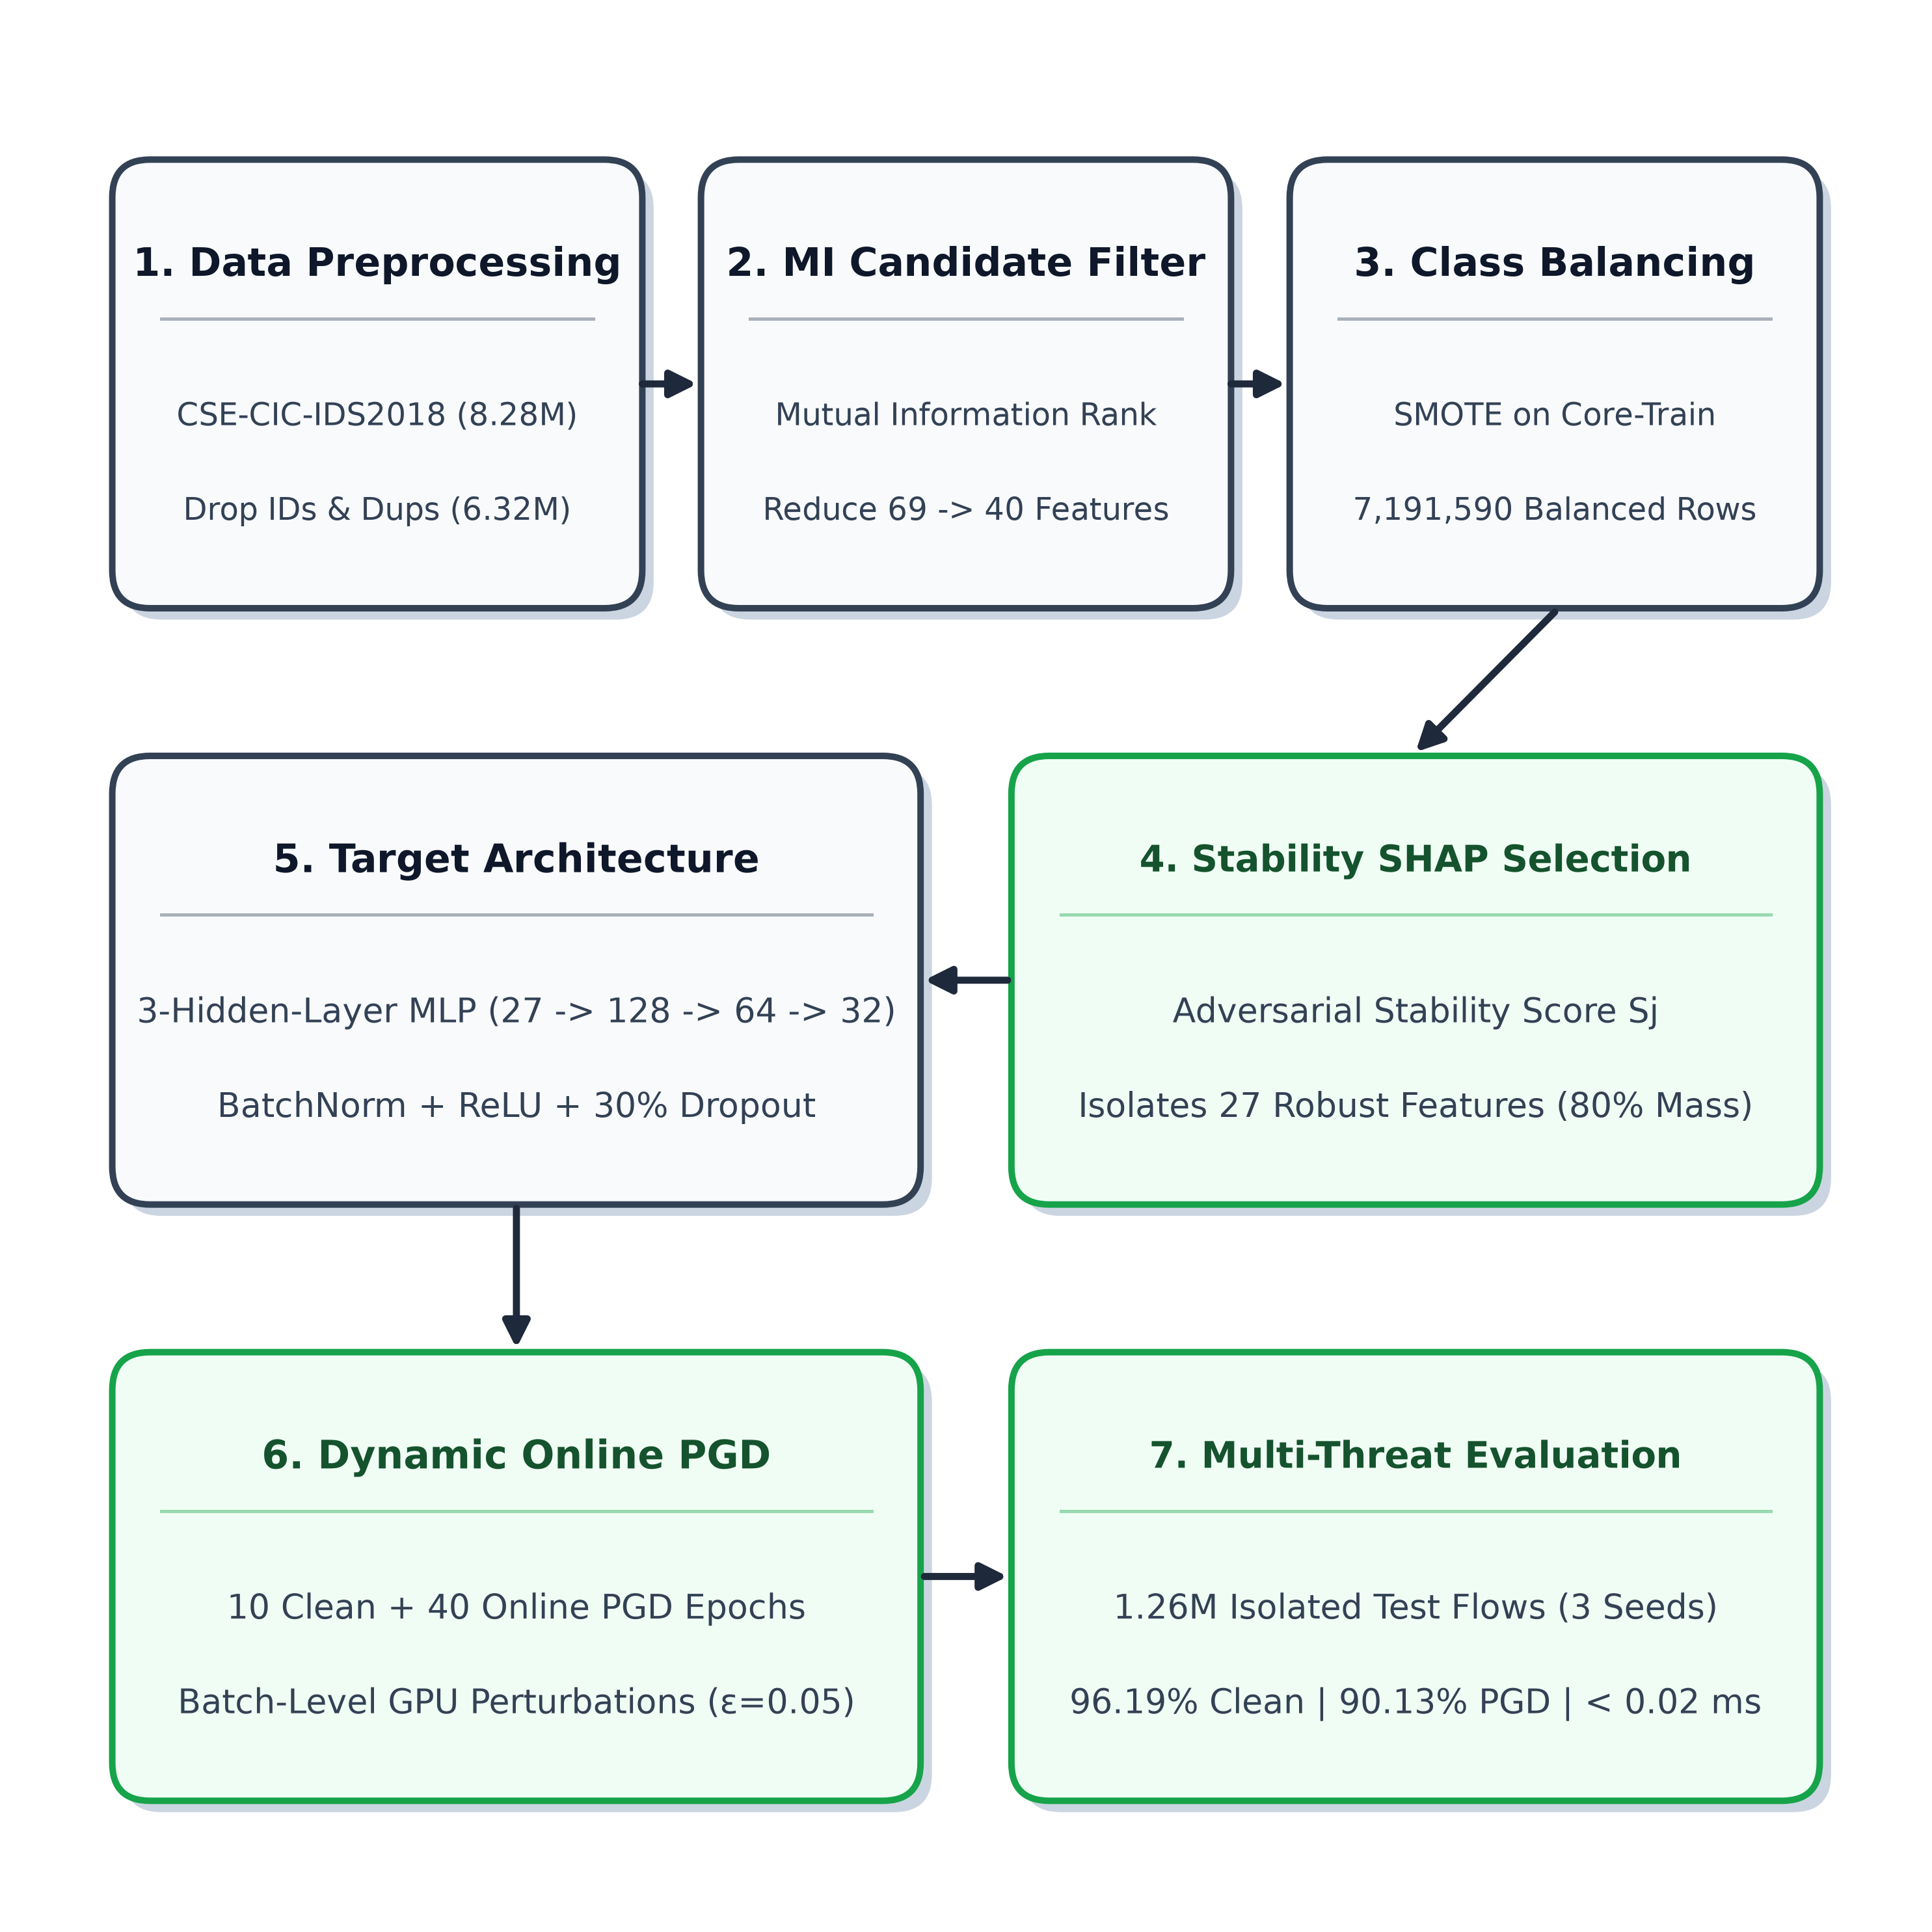
\includegraphics[width=\columnwidth]{flowchart.png}
\caption{End-to-end pipeline flowchart of the proposed defense framework.}
\label{fig:flowchart}
\end{figure}

\subsection{Dataset and Preprocessing}
We evaluate our methodology on the CSE CIC IDS2018 dataset by Dhoogla from Kaggle~\cite{ref2}. This contains 8,284,871 raw records across 10 CSV files. We selected this dataset because it contains diverse attack scenarios and high volume bidirectional flow statistics for enterprise network traffic.
\begin{itemize}
    \item Cleaning: We eliminated six identifier columns (Source IP, Destination IP, Flow ID, Source Port, Destination Port, and Timestamp) to keep the model from relying on identifying data. Object typed fields are converted to float32. We remove rows containing missing values, infinite values, zero variance columns, and duplicate records. This leaves 6,320,003 valid flows (4,994,159 benign [79.02\%] and 1,325,844 attack flows [20.98\%]).
    \item Partitioning: We apply a stratified 80/20 train test split. The test set (1,264,001 flows) is frozen for final evaluation. The remaining data is divided into a 90\% core training set (4,550,401 flows) and a 10\% validation set (505,601 flows).
    \item Encoding \& Scaling: One Hot Encoding for categorical protocol fields and StandardScaler normalization are fitted strictly on the core training set. They are then applied to the validation and test sets in transform only mode. This prevents data leakage and produces 69 numeric dimensions.
\end{itemize}

\subsection{Mutual Information Candidate Filtering}
Computing SHAP attributions across 69 dimensions on millions of records is computationally expensive. So we apply Mutual Information (MI)~\cite{ref12} on a randomly sampled 100,000 row subset of the core training set. The top 40 features with the highest statistical dependency with the class labels are retained. This reduces the feature space from 69 to 40.

\subsection{SMOTE Class Balancing}
The core training set has an approximate 4:1 class imbalance (3,595,795 benign vs.\ 954,606 attack flows). This imbalance can lead the defense model to focus more on the greater segment of benign class. We apply SMOTE~\cite{ref15} strictly to the 40 standardized MI features of the core training set. Since the features are standardized, SMOTE treats them as continuous numeric values during nearest neighbor interpolation. This produces a balanced core training set of 7,191,590 flows (3,595,795 per class). The validation and test sets are not resampled, so their natural class distributions are preserved.

\subsection{Adversarial Stability SHAP Feature Selection}
Standard feature selection methods rank features using clean data only. However, features with high predictive importance on clean data may have steep loss gradients and may become more sensitive to adversarial perturbations.

To select features that maintain stable importance under attack, we use the following four steps:
\begin{itemize}
    \item Calibration Model: A preliminary calibration MLP with a 40 dimensional input is trained on the balanced core training set for 20 epochs using Adam ($\eta=0.001$, batch size 2,048). A 3-hidden-layer Multi-Layer Perceptron (MLP) consisting of fully connected layers of size 128, 64, and 32, each followed by Batch Normalization, Rectified Linear Unit (ReLU) activations, and 30\% Dropout regularization, terminating in a 2 unit linear output layer for binary classification.
    \item Dual State Attribution Extraction: Using \texttt{shap.GradientExplainer} with 200 background samples drawn strictly from core train, the same 500 core training samples are analyzed in their clean state and then perturbed using 20 step PGD ($\epsilon=0.05$, $\alpha=0.005$). This produces paired mean absolute attributions $\bar{\phi}_j^{\text{clean}}$ and $\bar{\phi}_j^{\text{adv}}$.
    \item Adversarial Stability Score: Because $\bar{\phi}_j^{\text{clean}},\bar{\phi}_j^{\text{adv}}\ge0$, we define the Adversarial Stability Score $S_j\in[0,1]$ for each feature $j$:
    \begin{equation}
    S_j = 1 - \frac{\left|\bar{\phi}_j^{\text{clean}} - \bar{\phi}_j^{\text{adv}}\right|}{\max\left(\bar{\phi}_j^{\text{clean}} + \bar{\phi}_j^{\text{adv}}, 10^{-10}\right)}
    \end{equation}
    The numerator measures the change in attribution under attack. The denominator normalizes this change using the combined attribution values. The $10^{-10}$ term prevents division by zero. A score $S_j\approx1.0$ indicates stable feature importance under attack, while $S_j\approx0.0$ indicates a large attribution change.
    \item Selection Cutoff: Candidate features are sorted in descending order of $S_j$. We select features until reaching 80\% of the total cumulative stability mass ($\sum_{j=1}^{m} S_j \ge 0.80 \sum_{k=1}^{40} S_k$). This removes the less stable trailing features and selects the 27 most stable features ($40\to27$).
\end{itemize}

\subsection{Target Classifier Architecture}
After selecting the 27 stable features, the final target classifier is initialized and trained from scratch. The neural network is a fully connected Multi Layer Perceptron (MLP) with three hidden layers. The architecture maps the 27 input features through three sequential hidden dense layers of dimensions 128, 64, and 32. Each hidden transformation is followed by Batch Normalization to stabilize internal covariate shift across mini-batches, ReLU non-linear activations, and a 0.30 Dropout probability to prevent weight co-adaptation on synthetic SMOTE instances. The final linear projection yields two unnormalized logits for binary classification (Benign vs.\ Attack).

\subsection{Dynamic Online PGD Training}
To reduce the perturbation staleness found in static data augmentation, training uses two phases:
\begin{itemize}
    \item Phase 1: Clean Pretraining (10 Epochs): The model trains for 10 epochs on the clean balanced training set using standard cross entropy loss and Adam ($\eta=0.001$, batch size 2,048). This provides stable initial model weights before adversarial training.
    \item Phase 2: Dynamic Online PGD Training (40 Epochs): For the remaining 40 epochs, the model trains on both clean and dynamically generated adversarial samples. For each mini batch $(X_b,Y_b)$, the GPU generates fresh 5 step PGD perturbations ($k=5$, $\epsilon=0.05$, $\alpha=0.005$). The perturbations start with uniform random noise inside the $\epsilon$ ball and are clipped to the empirical training domain bounds $[l,u]$. The attacks are generated using the current model weights.
\end{itemize}
The total training loss gives equal weight to clean and adversarial cross entropy losses: $L_{\text{total}}=0.5L_{\text{clean}}+0.5L_{\text{adv}}$. New adversarial examples are generated for each training batch using the latest model weights. So the training process can adapt to changes in the decision boundary and reduce perturbation staleness.

To guarantee statistical validity and verify training reproducibility, the entire training pipeline is executed independently across three random seeds (42, 123, and 2024).

\subsection{Threat Model}
We evaluate the defense under an untargeted evasion threat model in standardized continuous feature space. The adversary aims to modify malicious network flows so that they are classified as benign while remaining within the $L_\infty$ evasion budget $\epsilon=0.05$. We consider three attack settings:
\begin{itemize}
    \item White Box Access: The attacker has full information of the model architecture, weights $\theta$, and loss gradients.
    \item Black Box Access: The attacker has query-only access to model output probabilities, evaluated via score-based random search (Square attack).
    \item Surrogate Transfer: Perturbations are generated using an independently trained wider surrogate MLP ($256\to128\to64\to2$) and transferred to the target model to evaluate cross model evasion.
\end{itemize}
All perturbations are clipped to the empirical training domain bounds $[l,u]$ to keep the modified features within the standardized feature range.

% ==============================================================
%  SECTION IV — RESULTS AND ANALYSIS
% ==============================================================
\section{Results and Analysis}
This section shows the evaluation findings on 1,264,001 frozen test flows from CSE-CIC-IDS2018 across three random seeds (42, 123, 2024). All metrics are reported as Mean $\pm$ Std. Attack Success Rate (ASR) is defined as the proportion of initially correctly classified clean samples that are misclassified after applying the perturbation.

\subsection{Clean Classification Performance}
We compare three model configurations on clean network traffic:
\begin{itemize}
    \item Undefended Baseline: Uses 15 features selected by Mutual Information, SMOTE class balancing, and standard clean SHAP. The model is trained only on clean data for 50 epochs.
    \item Static Defense~\cite{ref4}: Uses the same 15 feature representation and architecture as the baseline, with static offline adversarial retraining using pre computed attack samples.
    \item Proposed Defense: Uses 27 features selected through Adversarial Stability SHAP and two phase dynamic online PGD training.
\end{itemize}

\begin{table}[!t]
\caption{Clean Test Performance}
\label{tab:clean}
\centering
\begin{tabular}{@{}lccc@{}}
\toprule
\textbf{Metric} & \textbf{Baseline} & \textbf{Static} & \textbf{Proposed} \\
\midrule
Accuracy (\%) & 92.82 & 93.97 & 96.19 \\
F1-Score & 0.9303 & 0.9403 & 0.9620 \\
MCC & 0.8020 & 0.8257 & 0.8859 \\
Balanced Acc (\%) & 92.56 & 91.81 & 94.54 \\
\bottomrule
\end{tabular}
\end{table}

The proposed defense achieves a clean accuracy of 96.19\% $\pm$ 0.03\%, improving by 3.37 percentage points (pp) over the baseline (92.82\% $\pm$ 0.07\%) and 2.22 pp over the static defense (93.97\% $\pm$ 1.09\%)~\cite{ref4}. It also improves MCC to 0.8859 $\pm$ 0.0007 (+0.0839 over baseline 0.8020 $\pm$ 0.0013). As detailed in Table~\ref{tab:clean}, the proposed defense achieves a clean F1-score of 0.9620 $\pm$ 0.0003 and a balanced accuracy of 94.54\% $\pm$ 0.03\% (compared to 92.56\% $\pm$ 0.03\% and 91.81\% $\pm$ 2.09\% for the baseline and static defense). This demonstrates that dynamic adversarial training preserves high detection sensitivity across both normal and malicious flow distributions with high statistical stability.

\subsection{Adversarial Robustness under Standard Threat ($\epsilon=0.05$)}
Table~\ref{tab:adversarial} compares the models under white box, black box, and surrogate transfer attacks using an evaluation budget of $\epsilon=0.05$.

\begin{table}[!t]
\caption{Adversarial Robustness under Standard Threat (Accuracy, $\epsilon=0.05$)}
\label{tab:adversarial}
\centering
\begin{tabular}{@{}lccc@{}}
\toprule
\textbf{Attack} & \textbf{Baseline} & \textbf{Static} & \textbf{Proposed} \\
\midrule
FGSM & 84.20 & 84.32 & 92.67 \\
PGD-100 & 73.90 & 79.70 & 90.13 \\
Square & 82.00 & 85.40 & 91.83 \\
Transfer PGD & 79.23 & 86.73 & 94.13 \\
\bottomrule
\end{tabular}
\end{table}

Under PGD-100, baseline accuracy decreases by 18.92 pp to 73.90\% $\pm$ 2.43\% (ASR 20.14\%). In contrast, the proposed defense retains 90.13\% $\pm$ 1.20\% accuracy, outperforming the static defense (79.70\% $\pm$ 5.45\%, ASR 15.23\%) by 10.43 pp and reducing ASR to 6.05\%. Under single-step FGSM, the proposed defense reaches 92.67\% $\pm$ 1.56\% (ASR 3.62\%) compared to baseline 84.20\% $\pm$ 3.30\%. Under gradient-free Square attack, it maintains 91.83\% $\pm$ 1.07\% (ASR 5.27\%), and reaches 94.13\% $\pm$ 1.68\% against surrogate Transfer PGD (ASR 2.08\%). As shown in Fig.~\ref{fig:asr}, the proposed defense consistently reduces Attack Success Rate (ASR) across the evaluated threat formulations. PGD-100 ASR decreases from 20.14\% to 6.05\%, while transfer ASR decreases to 2.08\%. The confusion matrix in Fig.~\ref{fig:cm_pgd} also shows a low false alarm rate on benign traffic ($<$1\%). The proposed defense correctly classifies 90.13\% of adversarial attack flows under 100 step PGD evaluation.

\begin{figure}[!t]
\centering
\includegraphics[width=\columnwidth]{20_asr_all_models.png}
\caption{Attack Success Rate (ASR) comparison across threat categories for Baseline, Static Defense, and Proposed Defense.}
\label{fig:asr}
\end{figure}

\begin{figure}[!b]
\centering
\includegraphics[width=\columnwidth]{11_cm_proposed_pgd.png}
\caption{Confusion matrix of the proposed defense under 100-step PGD attack ($\epsilon = 0.05$) on 1,264,001 test flows.}
\label{fig:cm_pgd}
\end{figure}

\subsection{Generalization Across Unseen Attacks}
To examine whether the defense overfits to the 5 step PGD used during training, Table~\ref{tab:unseen} evaluates four unseen white box attacks at $\epsilon=0.05$.

\begin{table}[!t]
\caption{Robustness Against Unseen White Box Attacks (Accuracy \& ASR, $\epsilon=0.05$)}
\label{tab:unseen}
\centering
\begin{tabular}{@{}lccc@{}}
\toprule
\textbf{Attack} & \textbf{Trait} & \textbf{Accuracy} & \textbf{ASR} \\
\midrule
BIM & Sign Gradient & 91.37 & 4.76 \\
MIM & Momentum Memory & 91.05 & 5.09 \\
APGD-CE & Adaptive Decay & 88.55 & 7.70 \\
CW-$L_\infty$ & Margin Loss & 90.15 & 6.03 \\
\bottomrule
\end{tabular}
\end{table}

As detailed in Table~\ref{tab:unseen}, the proposed model maintains robust accuracy across all four unseen white-box attacks. This achieves 91.37\% $\pm$ 0.43\% on BIM (ASR 4.76\% $\pm$ 0.25\%), 91.05\% $\pm$ 1.85\% on MIM (ASR 5.09\% $\pm$ 1.77\%), 88.55\% $\pm$ 1.95\% on APGD-CE (ASR 7.70\% $\pm$ 1.88\%), and 90.15\% $\pm$ 1.21\% on CW-$L_\infty$ (ASR 6.03\% $\pm$ 1.03\%). This shows that the observed adversarial robustness generalizes across diverse gradient optimization objectives and is not overfitted to the specific 5-step PGD formulation used during training.

\subsection{Sensitivity Analysis and Boundary Diagnostics}
Across the three seeds, mean PGD 100 accuracy decreases from 94.47\% at $\epsilon=0.01$ to 93.35\%, 90.13\%, and 75.25\% at $\epsilon=0.03$, 0.05, and 0.10, respectively. This gradual decrease is consistent with the expected effect of stronger perturbations and does not show obvious signs of gradient masking. Increasing PGD iterations from 20 to 200 at $\epsilon=0.05$ changes accuracy from 91.40\% to 90.13\%. This provides further evidence against obvious gradient masking. Fig.~\ref{fig:attack_sweeps} shows model accuracy under different perturbation budgets $\epsilon \in [0.01, 0.10]$ and PGD iteration steps from 20 to 200. The results show no sudden drop in accuracy and indicate stable attack convergence.

\begin{figure}[!t]
\centering
\includegraphics[width=\columnwidth]{15_attack_sweeps.png}
\caption{Model accuracy across varying perturbation budgets $\epsilon \in [0.01, 0.10]$ and PGD iteration steps from 20 to 200.}
\label{fig:attack_sweeps}
\end{figure}

DeepFool~\cite{ref9} uses an unconstrained perturbation objective. Therefore, its results are treated as a boundary distance diagnostic rather than a direct comparison with $\epsilon$ bounded attacks. For the proposed defense, successful DeepFool attacks required a mean $L_\infty$ perturbation of 2.3238 and a median of 1.0064. Only 2.67\% of successful perturbations occurred within the operational $\epsilon=0.05$ budget, while 97.33\% exceeded it. This suggests that many successful boundary crossings required perturbations larger than the operational budget. Fig.~\ref{fig:boundary} illustrates the DeepFool unconstrained perturbation distance distribution. This highlights that 97.33\% of samples require perturbations exceeding the operational $\epsilon = 0.05$ threshold to cross the decision boundary.

\begin{figure}[!b]
\centering
\includegraphics[width=\columnwidth]{16_boundary_diagnostics.png}
\caption{DeepFool unconstrained perturbation distance distribution and operational $\epsilon = 0.05$ threshold.}
\label{fig:boundary}
\end{figure}

\subsection{Statistical Stability and Overhead}
\begin{itemize}
    \item Repeatability: The small standard deviations across seeds ($\pm$0.03\% on clean data and $\pm$1.20\% under PGD 100) indicate consistent performance under the evaluated settings.
    \item Computational Overhead and Hardware Specifications: Experiments were conducted on a commodity PC with an AMD Radeon RX 7600 GPU (8 GB GDDR6 VRAM), 32 GB system RAM, and PyTorch (ROCm 7.2.1). For the proposed defense on 7.19M balanced flows with a batch size of 2,048, Phase 1 clean pretraining required $\sim$13 seconds per epoch, while Phase 2 dynamic online PGD required $\sim$99 seconds per epoch, including on the fly 5 step GPU attack generation. Complete target model training took approximately 69.3 minutes (4,160 s) per seed, totaling $\sim$3.5 hours across all three seeds. The measured average amortized inference time was below 0.02\,ms per flow under this hardware configuration.
\end{itemize}

% ==============================================================
%  SECTION V — COMPARATIVE STUDY AND CONCLUSION
% ==============================================================
\section{Comparative Study and Conclusion}

\subsection{Comparative Discussion}
Compared with recent adversarial NIDS studies~\cite{ref4,ref11,ref13}, the proposed framework addresses key issues in feature selection and training:
\begin{itemize}
    \item Feature Stability: Prior works (e.g., Holla et al.~\cite{ref4}, Hashemi et al.~\cite{ref13}) mainly select features using clean data importance. Our approach uses the Adversarial Stability Score to rank features and selects 27 features with more stable SHAP attributions under adversarial perturbation.
    \item Adversarial Generalization: Static offline retraining~\cite{ref4} can suffer from perturbation staleness as the decision boundary changes, resulting in lower PGD-100 accuracy (79.70\%). The proposed framework generates fresh perturbations for each mini batch during dynamic online PGD training and achieves 90.13\% PGD 100 accuracy, while also achieving 96.19\% clean accuracy.
\end{itemize}

\subsection{Conclusion and Future Work}
This paper demonstrated an integrated defense framework for cloud intrusion detection combining adversarial-stability SHAP feature selection with dynamic online PGD training. Evaluated on 1,264,001 test flows from CSE-CIC-IDS2018 across three random seeds, the defense achieved 96.19\% clean accuracy and 90.13\% PGD 100 accuracy. It also showed resistance against unseen white box, black box, and transfer attacks. The measured average inference time was below 0.02\,ms per flow under the experimental hardware configuration.

Limitations and Future Work: While the evaluation shows improved empirical robustness under the tested threat settings in standardized continuous feature space, future work will investigate mapping continuous flow perturbations back to packet level network constraints, including PCAP reconstruction and protocol header validity. Future work will also evaluate the framework for multi class intrusion detection and emerging zero day attack families.

% ==============================================================
%  REFERENCES
% ==============================================================
\begin{thebibliography}{15}

\bibitem{ref1}
I.~Sharafaldin, A.~H.~Lashkari, and A.~A.~Ghorbani, ``Toward generating a new intrusion detection dataset and intrusion traffic characterization,'' in \emph{Proc. ICISSP}, 2018, pp.~108--116.

\bibitem{ref2}
D.~Dhoogla, ``CSE-CIC-IDS2018 on AWS,'' Kaggle Dataset, 2020. [Online]. Available: \url{https://www.kaggle.com/datasets/dhoogla/csecicids2018}

\bibitem{ref3}
I.~J.~Goodfellow, J.~Shlens, and C.~Szegedy, ``Explaining and harnessing adversarial examples,'' in \emph{Proc. ICLR}, 2015.

\bibitem{ref4}
A.~Holla, G.~Polepalli, and K.~Sasikumar, ``Adversarial threats to cloud IDS: Robust defense with adversarial training and feature selection,'' \emph{IEEE Access}, vol.~13, pp.~1--15, 2025.

\bibitem{ref5}
A.~Madry, A.~Makelov, L.~Schmidt, D.~Tsipras, and A.~Vladu, ``Towards deep learning models resistant to adversarial attacks,'' in \emph{Proc. ICLR}, 2018.

\bibitem{ref6}
S.~M.~Lundberg and S.-I.~Lee, ``A unified approach to interpreting model predictions,'' in \emph{Proc. NeurIPS}, 2017, pp.~4765--4774.

\bibitem{ref7}
F.~Croce and M.~Hein, ``Reliable evaluation of adversarial robustness with an ensemble of attacks,'' in \emph{Proc. ICML}, 2020, pp.~2206--2216.

\bibitem{ref8}
N.~Carlini and D.~Wagner, ``Towards evaluating the robustness of neural networks,'' in \emph{Proc. IEEE S\&P}, 2017, pp.~39--57.

\bibitem{ref9}
S.-M.~Moosavi-Dezfooli, A.~Fawzi, and P.~Frossard, ``DeepFool: A simple and accurate method to fool deep neural networks,'' in \emph{Proc. CVPR}, 2016, pp.~2574--2582.

\bibitem{ref10}
M.~Andriushchenko, F.~Croce, N.~Flammarion, and M.~Hein, ``Square Attack: A query-efficient black-box adversarial attack via random search,'' in \emph{Proc. ECCV}, 2020, pp.~484--501.

\bibitem{ref11}
X.~Zhou, W.~Liang, J.~Wang, K.~I.~Wang, and L.~Y.~Qi, ``Certified adversarial robustness for intrusion detection in cyber-physical systems,'' \emph{IEEE Trans. Dependable Secure Comput.}, vol.~20, no.~4, pp.~3202--3214, 2023.

\bibitem{ref12}
A.~Kraskov, H.~St\"{o}gbauer, and P.~Grassberger, ``Estimating mutual information,'' \emph{Phys. Rev. E}, vol.~69, no.~6, p.~066138, 2004.

\bibitem{ref13}
M.~Hashemi, G.~Cusack, and E.~Keller, ``Improving intrusion detection robustness against adversarial evasion,'' \emph{Comput. Secur.}, vol.~138, p.~103648, 2024.

\bibitem{ref14}
G.~Apruzzese, M.~Andreolini, L.~Ferretti, M.~Marchetti, and M.~Colajanni, ``Modeling realistic adversaries in cybersecurity,'' \emph{ACM Comput. Surv.}, vol.~55, no.~14, pp.~1--39, 2023.

\bibitem{ref15}
N.~V.~Chawla, K.~W.~Bowyer, L.~O.~Hall, and W.~P.~Kegelmeyer, ``SMOTE: Synthetic Minority Over-sampling Technique,'' \emph{J. Artif. Intell. Res.}, vol.~16, pp.~321--357, 2002.

\end{thebibliography}

\end{document}
